
\documentclass[man,noapacite]{apa2}
\usepackage{amsmath}
\usepackage{booktabs}
\usepackage{apacite2}
\usepackage{fullpage,rotating}
\usepackage{pslatex}
\usepackage{amssymb}

\title{\vspace{-16ex}Using rational speech act models of pragmatic reasoning to understand human behavior in reference games}

\fiveauthors{Michael C. Frank}{Andr\'es G\'omez Emilsson}{Alex J. Stiller}{Christopher G. Potts}{Noah D. Goodman}
\fiveaffiliations{Department of Psychology, Stanford University}{Department of Psychology, Stanford University}{Department of Linguistics, University of California, San Diego}{Department of Linguistics, Stanford University}{Department of Psychology, Stanford University}

\shorttitle{Rational speech act models}
\rightheader{Rational speech act models}


\newcommand{\argmax}{\operatornamewithlimits{argmax}}

\acknowledgements{Thanks to Avery Katko, Benjamin Gittleson, Paul Mains for assistance in data collection and design for Experiments XYZ. Thanks to Roger Levy for much valuable discussion and the design of the ``odd man out'' stimulus. Generous thanks to Allison Kraus for designing the stimuli used here.  Some of these ideas and experimental designs were presented in substantially different form in \citeA{stiller2011}; data from Experiment XYZ were presented in \cite{vogel2013}. We acknowledge funding from ONR and Merck Family Foundation ...

~

\noindent Please address correspondence to Michael C. Frank, Department of Psychology, Stanford University, 450 Serra Mall (Jordan Hall), Stanford, CA, 94305, tel: (650) 724-4003, email: \texttt{mcfrank@stanford.edu}.}


\abstract{Human communication is almost always underspecified. Nevertheless, most communication takes place in a context where otherwise ambiguous messages can be decoded. A key part of this process of pragmatic disambiguation for a listener is reasoning about the speaker's intentions; but a smart speaker will consider what kind of reasoning the listener is going to do and design her message with that in mind. A variety of recent work on formal pragmatics has made use of recursive systems of this type, based on a generalized notion of ``signaling systems.'' Here we show that these systems can be written as special cases of a probabilistic recursive reasoning model, with a small number of choice-points, including the depth of the recursion possible for human communicators and whether they interpret messages greedily. We present experimental data that bear on these decisions.}

\begin{document}
\maketitle                            


\section{Introduction}



\section{Formal Framework}
\label{sec:models}

In this section, we describe formal details of the ``rational speech act'' model. As described above, this model has been presented previously \cite{frank2012,goodman2013}. Our goal here is to provide a more comprehensive formal presentation. This presentation allows us to highlight choice-points in the model that we test below; in addition, it illuminates parallels and differences with other formal models in this space (specific comparisons are given in Appendix \ref{app:equivalences}).

% We introduce a notation for signaling games and other recursive reasoning problems \cite{golland2010,franke2012,frank2012,goodman2013}. This notation system allows us to define a set of recursive models; we show that a set of recent systems for pragmatic reasoning can be written within this system. As a consequence, they are equivalent to one another modulo three design decisions: 


\subsection{Preliminaries}

A reference game under our definition is a game in which a speaker $S$ and listener $L$ collaborate in a context $C$ to identify a particular object in the context, known as the speaker's intended referent $r_S \in C$. The game has two parts. First the speaker chooses an utterance $w$ based on vocabulary $V$; this process can be as simple as selection from a list or as complex as generation from a grammar. Next the listener guesses a referent $r_L \in C$ after hearing $w$. The game is won if $r_S=r_L$.

There is a ``contextual salience'' distribution $\sigma$ over the objects ${o_1 ... o_n} \in C$, which is mutually known to both speaker and hearer. This distribution picks out those objects in the context which are more or less likely to be talked about, either because of their intrinsic perceptual or conceptual noteworthiness, or because of some prior history between speaker and listener (e.g. one object having been talked about previously). 

There is also a mutually-known semantics for the vocabulary of possible words (messages) $w$ that a speaker can send.  Each message can be described as a Kronecker $\delta$ function that applies to referents and returns 1 if the message is true of that referent, 0 otherwise. 

\subsection{The model}

We define the RSA model in terms of two agents, a listener $L$ and a speaker $S$. Their goals are to reason about one another so that they are able to transmit information efficiently. $L$ reasons abut what word $S$ would have said to describe a particular referent; $S$ reasons about what interpretation $L$ would give to a particular message. Each of these agents uses Bayesian inference to reason about the other's likely actions. 

So we can define:

\begin{equation}
  \begin{array}{r@{}l}
    \label{eq:agents}
    P_L(r_S | w, C) & \propto P_S (w | r_S, C) P(r_S)\\
    P_S(w | r, C) & \propto P_L (r_S | w, C)  
  \end{array}
\end{equation}

\noindent where $P(r_S)$ is a prior distribution over referents, which we discuss extensively below. In principle, we could also add a prior on words, $P(w)$, but for simplicity here we assume that $P(w) \propto 1$ and do not discuss it further. 

The two agents in Equation \ref{eq:agents} are defined recursively and so individual probabilities are undefined unless the recursion ends. Thus, we define a further agent, $L_0$, the ``literal listener,'' who grounds the recursion:

\begin{equation}
P_{L_0} (r_S | w, C) \propto \begin{cases} \frac{1}{\sum_{r \in C} \delta_w(r)} &\mbox{if } \delta_w(r_s) = 1 \\ 
0 & \mbox{otherwise.} \end{cases} 
\end{equation}

\noindent In other words, agent $L_0$ simply chooses uniformly between available referents that are consistent with $w$. 

With these agents defined, we can then imagine variations on this model where $L$ reasons about $S$, who in turn reasons about $L_0$. 

See Appendix \ref{app:alternative}

\subsection{Choice-points}

\begin{enumerate}
\item The depth of the recursion between speaker and listener,
\item Whether the recursion starts with speaker or listener,
\item The decision rule chosen by speaker and listener (soft vs. hard maximization), and 
\item Whether the model includes a term indicating the prior probability of a referent being talked about.
\end{enumerate}

\noindent We show equivalences of various special cases of this notation to the systems described in these prior reports.

\subsection{An example}

% \begin{figure}[t]
%   \begin{center} 
%     \includegraphics[width=4.5in]{figures/bugs.jpg} 
%     \caption{\label{fig:ex} An example stimulus for our 3 objects, 3 features experiment. Inferring that ``tail'' referred to C is a depth-0 computation, inferring that ``feet'' referred to A is a depth-1 computation, and inferring that ``horns'' referred to B is a depth-2 computation.} 
%   \end{center} 
% \end{figure}

We work through an example computation on the stimulus shown in Figure \ref{fig:ex}, using the J\"ager \cite{jaegerinpress} version of the model described above (for simplicity and finite convergence): $L^*(S^*(L^*(S(C^T))))$. The object by feature matrix $C$ has as its columns the messages ``tail,'' ``horns,'' and ``feet'' and the objects A, B, and C as its rows.:

\begin{equation}
C= \left(
    \begin{array}{ccc}
      0 & 0 & 1 \\
      0 & 1 & 1\\
      1 & 1 & 0 
    \end{array} 
  \right)
\end{equation}

The corresponding speaker matrix $S(C^T)$ is inverted, with messages as rows and objects as columns: 

\begin{equation}
E = \left(
    \begin{array}{ccc}
      0 & 0 & 1 \\
      0 & .5 & .5\\
      .5 & .5 & 0 
    \end{array} 
  \right)
\end{equation}

It is already clear that ``tail'' is true only of object C, thus the interpretation of ``tail'' reaches depth 0. Now we perform a set of renormalizations to lead to the next level of recursion:

\begin{equation}
L^*(S(C^T)) = \left(
    \begin{array}{ccc}
      0 & 0 & 1 \\
      0 & .5 & .5\\
      1 & 0 & 0 
    \end{array} 
  \right)
\end{equation}

Now, at depth 1, the message ``feet'' is found to refer to object A. A final round of recursion leads to depth 2, where ``horns'' is found to refer to object B:

\begin{equation}
L^*(S^*(L^*(S(C^T)))) = \left(
    \begin{array}{ccc}
      0 & 0 & 1 \\
      0 & 1 & 0\\
      1 & 0 & 0 
    \end{array} 
  \right)
\end{equation}

We now say that the model has ``converged''---that is, further iteration will not lead to changes in state.

\subsection{Status of the model}

%%% Local Variables: 
%%% TeX-master: "pragmods"
%%% End:


\section{General Experimental Methods}

This section describes the methods used in the experiments reported below. Our goal was to create a general method for measuring pragmatic inferences in simple reference games. Our taking-off point is two previous studies in which simple feature-based displays allowed measurement of pragmatic reasoning in grounded contexts \cite{frank2012,stiller2014}. In what follows we describe some of the general features of these displays and the experiments that use them.
% In the experiments that follow we attempt to demonstrate that these signaling games provide a useful tool for measuring pragmatic reasoning. 

\subsection{Participants}

One challenge of pragmatic communication experiments is that repeated communication within a signaling game is very likely to influence responding \cite<e.g.,>{brennan1996}. For this reason, we adopted a massively between-subjects approach, where each participant answered exactly one relevant question.

We adopted a general standard of 50 independent participants per cell, based on the tradeoff between cost and the desired precision of measurements. With samples of N=50 participants making binary decisions, we could assume 95\% confidence intervals with width .24 at their widest; doubling the sample size to N=100 per cell would only reduce width to .18. While not every experiment reflects this precise standard due to idiosyncrasies of recruitment exclusion, we have tried to maintain approximately this standard throughout. 

All of the experiments described here were run on Amazon's Mechanical Turk crowdsourcing service, between Fall 2013 and Spring of 2015. In general, each experiment was run as an independent human intelligence task (HIT); a few were posted as multiple hits for convenience or due to experimenter error. In all cases, we remove duplicated workers from the samples, so that data in each experiment represent a set of unique judgments by distinct participants. 

In addition to excluding duplicated participants, we also excluded participants who failed manipulation checks (see below). Table \ref{tab:expts} gives details of participants for each experiment. 

\subsection{Stimuli}

We created a set of six base domains that had features that could easily be added independently: faces (pictured in Figure \ref{fig:ex}), boats, pizzas, sundaes, snowmen, and christmas trees. We created slightly different versions of each base so that they would appear to be unique (e.g., by varying the proportions or color tone of the face). We then were able to add features to each of these programmatically (with most experiments using two features but some using three). Faces were supplemented with hats, glasses, and mustaches; boats had motors, sails, and cabins; pizzas had olives, peppers, and mushrooms; sundaes had whipped cream, chocolate, and cherries on top; snowmen had mittens, hats, and scarves; and christmas trees had lights, ornaments, and stars on top.

\subsection{Procedure}

Participants viewed the experiment within a browser window. The first screen of the experiment presented a basic description of the paradigm and asked for informed consent. The second screen of the experiment presented the interlocutor, Bob (a cartoon picture of a man), and noted that he liked to do activities with the base item (e.g., visit friends or sail boats). In experiments with familiarization stimuli (e.g., \exptref{exp:prior-baserate}), nine familiarization images were presented on this screen. 

The third screen was the key screen: it presented the experimental stimulus (a set of base items augmented with features, representing the signaling game of interest) at the top of the screen. Below each stimulus a letter was displayed. From left to right: A, B and C. In all experiments except for \exptref{exp:prelims-mc}, two manipulation check questions were asked directly below the display using text entry boxes (e.g. ``how many boats have cabins?''). Below this was the prompt, e.g. ``Bob can only say one word to communicate with you and he says: {\it glasses}. Click below on the option that represents the friend that you think Bob is talking about.'' Below this was a set of buttons labeled A, B and C for the participant to indicate which of the three options they thought the speaker was referring to. A final screen asked participants the following: ``Who did you meet in this survey?'',  ``What was this survey about?'' and ``Any other comments for us?'' Optionally, participants could also provide their age and gender, but finishing the experiment was not contingent on doing this.

Note that in the first set of experiments, we manipulate a number of these experimental choices, including the dependent variable, the use of the manipulation check, and the linguistic framing of Bob's utterance. Our description here reflects the defaults used in the majority of the experiments we report. 



% Minor stuff:

% Prelims measures has four items

% Size and sequence have no manipulation check 

%%% Local Variables: 
%%% TeX-master: "pragmods"
%%% End:


\begin{table}[ht!]
\caption{Organization of the experiments reported here.}
\begin{tabular}{cllllll}
\hline
Expt. \# & Sequence & Experiment & $N_{total}$ & $N_{include}$ & Summary \\
\hline
1 & Prelims & Dependent variable & 689 & 629 & Forced choice yields best DV \\
2 & & Manipulation check & 580 & 536 & Manipulation check does not create effect \\
3 & Prior & Base rate prior manipulation & 800 & 525 & Base rate affects inference \\
5 &  & Linguistic framing & & & Linguistic valence affects inference\\
6 &  & Perceptual salience framing & TODO & & Perceptual salience doesn't change inference\\
7 & Levels & Level of inference & 320 & 280 & Level 2 difficult for participants \\
8 &    & Levels prior &  &  & TODO \\
9 &    & Twins & 120 & 106  & Hard to get non-literal readings\\
10 &    & Oddman & 200 & 182  & Hard to get non-literal readings\\
11 & Size  & Distractors & 1300 & 1224  & \\
12 & Sequences & Level 1 & & & Limited sequential effect, no transfer \\
13 & & Level 1 x3 & & & No repetion effects \\
14 & & Level 2 & & & Strong sequence effect for level 2 \\
15 & Production & & & & \\
16 & & & & & \\
17 & & & & & \\


\hline
\end{tabular}
\end{table}

\section{Methodological preliminaries}
% prelims


% DV
% manipulation check
% linguistic framing - 

\section{Levels of recursion}
% levels

\section{Prior measurement}
% prior

\section{Prior manipulations 1: Base-rate manipulations}
% prior-baserates




\section{Prior manipulations 2: Linguistic manipulations}
% prior-language

\section{Sequential effects}
% sequences

\section{Tests of the speaker model}
% speakers

\section{Varying matrix size}
% size

\section{Non-linguistic equilibria}
% equilibria

\section{Model fits and model comparison}
\label{sec:models}

In the experiments reported above, we see strong evidence that participants are engaging in reasoning that goes beyond the simple semantic interpretation of messages. Instead, they appear to be making inferences about reference in context that have the character of pragmatic reasoning---considering inferential alternatives that a speaker could have said. In this section, we test the ability of the RSA model to describe human behavior in these experiments. 

We are well aware of the difficulties surrounding reasoning from a good fit alone \cite{roberts2000}. In a nutshell, any model must both show that it \emph{can} predict the data that actually occurred and \emph{cannot} predict the data that did not occur. The flexibility of the theory is thus of critical importance in understanding its performance. The RSA model as stated here and earlier contains a relatively small number of parameters, however: primarily $n$ (the depth of recursion) and $\alpha$, the greed parameter in the choice rule. 

 \begin{figure}[t]
  \centering
  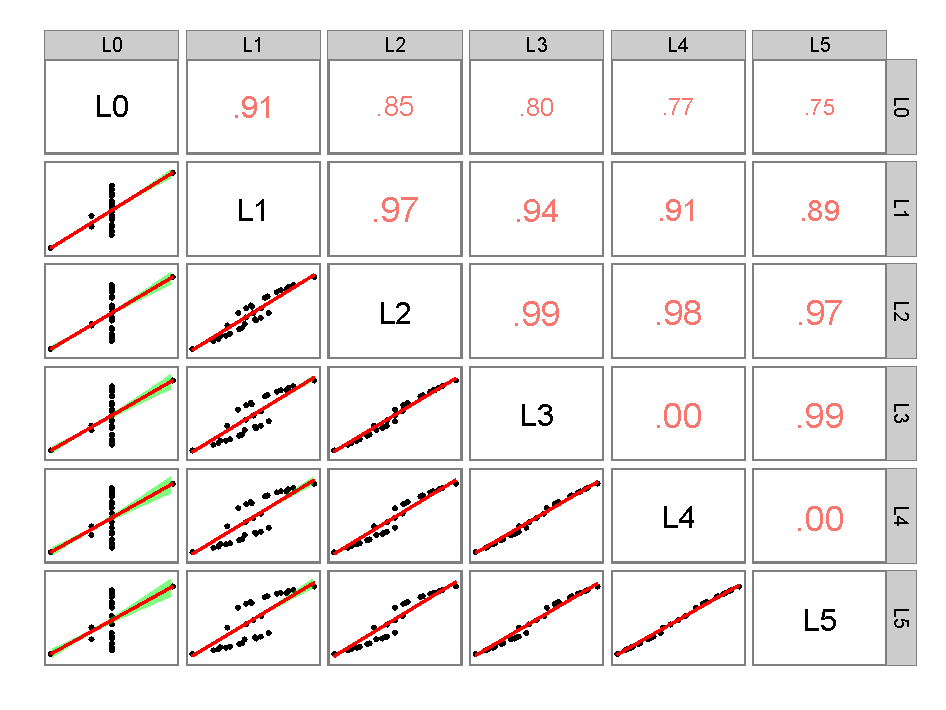
\includegraphics[width=6in]{../plots/models-2.pdf}
  \caption{\label{fig:models-2} Model identifiability simulation results. Each plot on the lower triangle shows model predictions for one model plotted by predictions for another. Each dot is an experimental condition, with trend lines showing simple linear regression with 95\% confidence intervals. Each plot on the upper triangle shows the pearson correlation value between those two models. Models with higher levels of recursion are very difficult to distinguish from one another.}
\end{figure}


 \begin{figure}[t]
  \centering
  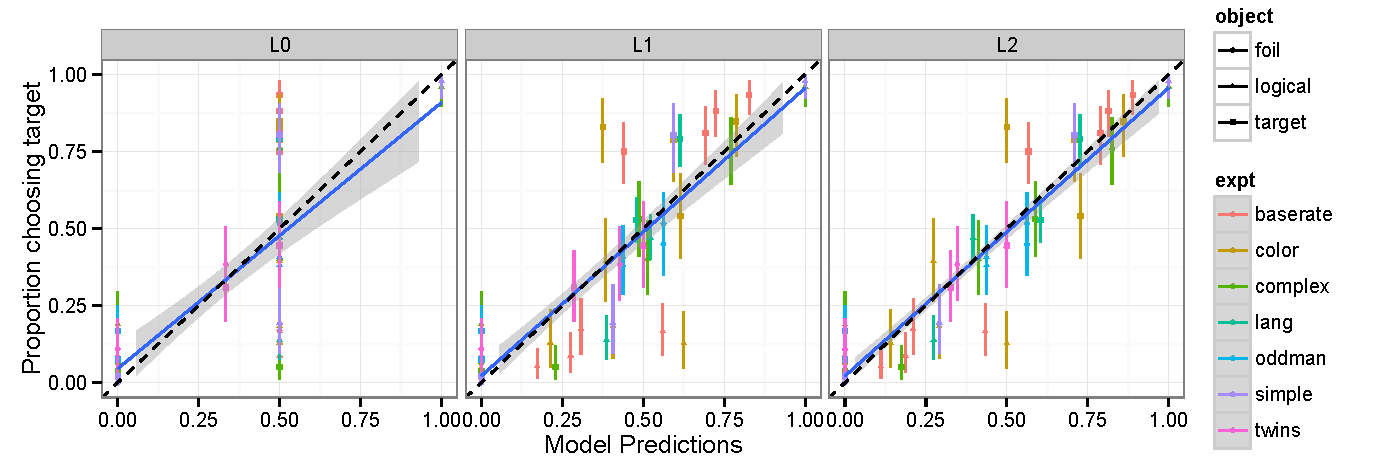
\includegraphics[width=6in]{../plots/models-1.pdf}
  \caption{\label{fig:models-2} Full model fit to data for $L_0$, $L_1$, and $L_2$. Each point represents proportions choosing a particular target object in an experimental condition. The diagonal dashed line shows perfect fit, and the blue solid line shows a line of best fit with 95\% confidence intervals.}
\end{figure}

In our first analysis, we 


\subsection{Identifiability}

%%% Local Variables: 
%%% TeX-master: "pragmods"
%%% End:


\section{General Discussion}


\newpage

\bibliographystyle{apacite}
\bibliography{pragmods}

\theappendix

\section{Equivalences to other models}
\section{Equivalences}

The model we describe above has as its special case several previous systems; in what follows we show these equivalences, as they motivate our experiment below.

\subsection{J\"ager (to appear)}

The system described here is a restatement and generalization of the Iterated Best Response model described in J\"aeger's work \cite{jaegerinpress}. That work notates $S(C^T)$ as $\sigma$, and proposes an algorithm in which recursive applications of $L^*$ and $S^*$ are made until $X = L(S(X))$. 

\subsection{Frank \& Goodman (2012)}

In recent work, Frank \& Goodman \cite{frank2012} described a utility-theoretic derivation of a similar framework. They start with the idea that speakers choose messages relative to their utility with respect to the number of bits of information they would send to a simple, truth-functional listener; this formulation reduced to

\begin{equation}
P(w|r_S,C) = \frac{|w|^{-1}}{\displaystyle \sum_{w' \in W} {|w'|^{-1}}},
\end{equation}

where $|w|$ indicated the number of objects to which $w$ could refer. The associated listener probability was given by Bayesian inference from the speaker's likelihood and a prior term $P(r_S)$:

\begin{equation}
\label{eq:fg}
% P(r_S | w, C) \propto P(w | r_S, C) P(r_S).
P(r_S | w, C) 
= \frac{P(w | r_S, C) P(r_S)}{\displaystyle \sum_{r' \in C}{P(w | r', C) P(r')}} =
\frac{\frac{\displaystyle |w|^{-1}}{\displaystyle \sum_{w' \in W} {|w'|^{-1}}}P(r_S)}{\displaystyle \sum_{r' \in C}{\frac{|w|^{-1}}{\displaystyle \sum_{w' \in W} {|w'|^{-1}}}P(r')}}.
% \frac{|w|^{-1}}{\displaystyle \sum_{w' \in W} {|w'|^{-1}}}
\end{equation}

Working from our definitions, this formulation is equivalent to $L_B(S(L(C)))$. We can rewrite $L(C_{o,w})$ using the same notation as above, with $|w|$ as the number of objects to which a word refers. This allows us to write 

\begin{eqnarray*}
% L(C_{o,w}) = \frac{C_{o,w}}{\displaystyle\sum_{o' \in C} C_{o',w}} = |w|^{-1} \\
S(L(C_{o,w})) &=& \frac{|w|^{-1}}{\displaystyle \sum_{w' \in V(C)} |w|^{-1}} \mbox{, and} \\
L_B(S(L(C_{w,o}))) &=& \frac{ \frac{\displaystyle |w|^{-1}}{\displaystyle \sum_{w' \in V(C)} |w|^{-1}}P(o)}{\displaystyle\sum_{o' \in C}  \frac{|w|^{-1}}{\displaystyle \sum_{w' \in V(C)} |w|^{-1}}P(o')},
\end{eqnarray*}

which is equivalent to Equation \ref{eq:fg}.

\subsection{Other work}

Golland, Liang, and Klein \cite{golland2010} describe a similar system based on \cite{jaegerinpress}, in which they call $S(C^T)$ the ``reflex speaker'' and $S(L(C))$ the ``reasoned speaker.'' Benz \cite{benz2005b} describes a game-theoretic system that is similar to $S(L(C))$. 

\subsection{An example}

% \begin{figure}[t]
%   \begin{center} 
%     \includegraphics[width=4.5in]{figures/bugs.jpg} 
%     \caption{\label{fig:ex} An example stimulus for our 3 objects, 3 features experiment. Inferring that ``tail'' referred to C is a depth-0 computation, inferring that ``feet'' referred to A is a depth-1 computation, and inferring that ``horns'' referred to B is a depth-2 computation.} 
%   \end{center} 
% \end{figure}

We work through an example computation on the stimulus shown in Figure \ref{fig:ex}, using the J\"ager \cite{jaegerinpress} version of the model described above (for simplicity and finite convergence): $L^*(S^*(L^*(S(C^T))))$. The object by feature matrix $C$ has as its columns the messages ``tail,'' ``horns,'' and ``feet'' and the objects A, B, and C as its rows.:

\begin{equation}
C= \left(
    \begin{array}{ccc}
      0 & 0 & 1 \\
      0 & 1 & 1\\
      1 & 1 & 0 
    \end{array} 
  \right)
\end{equation}

The corresponding speaker matrix $S(C^T)$ is inverted, with messages as rows and objects as columns: 

\begin{equation}
E = \left(
    \begin{array}{ccc}
      0 & 0 & 1 \\
      0 & .5 & .5\\
      .5 & .5 & 0 
    \end{array} 
  \right)
\end{equation}

It is already clear that ``tail'' is true only of object C, thus the interpretation of ``tail'' reaches depth 0. Now we perform a set of renormalizations to lead to the next level of recursion:

\begin{equation}
L^*(S(C^T)) = \left(
    \begin{array}{ccc}
      0 & 0 & 1 \\
      0 & .5 & .5\\
      1 & 0 & 0 
    \end{array} 
  \right)
\end{equation}

Now, at depth 1, the message ``feet'' is found to refer to object A. A final round of recursion leads to depth 2, where ``horns'' is found to refer to object B:

\begin{equation}
L^*(S^*(L^*(S(C^T)))) = \left(
    \begin{array}{ccc}
      0 & 0 & 1 \\
      0 & 1 & 0\\
      1 & 0 & 0 
    \end{array} 
  \right)
\end{equation}

We now say that the model has ``converged''---that is, further iteration will not lead to changes in state.



\end{document}

